\documentclass{article}
\twocolumn
\usepackage[utf8]{inputenc}
\usepackage{geometry}
\usepackage{amsmath}
\usepackage{amsthm}
\usepackage{mathtools}
\usepackage{commath}
\usepackage{tikz}

\title{\textbf{\Huge Assignment 1}}
\author{\large H.N Srikanth - SM21Mtech12012}

\date{August 2021}

\begin{document}

\providecommand{\mbf}{\mathbf}

\newcommand{\myvec}[1]{\ensuremath{\begin{pmatrix}#1\end{pmatrix}}}
\let\vec\mathbf

\maketitle

\section*{Chapter II, Examples II}
\textbf{Q22 (iii)}
\textbf{Find the conditions that the four points}
\begin{align}
\myvec{x_1\\y_1}, \myvec{x_2\\y_2},
\myvec{x_3\\y_3}, \myvec{x_4\\y_4}
\end{align}
\textbf{ may be the vertices of a rhombus.}\\

\textbf{Solution :}

The given points are\\
$$\vec{A} = \myvec{x_1\\y_1}, \vec{B} =\myvec{x_2\\y_2},$$
$$\vec{C} =\myvec{x_3\\y_3}, \vec{D} =\myvec{x_4\\y_4},$$\\
Conditions for the given four points to be the vertices of a rhombus are:
\begin{enumerate}
  \item If opposite sides are parallel and
  \item If diagonals are perpendicular .
\end{enumerate}
if

\begin{equation}\label{first_equation}
(\vec{A}-\vec{B} ) = k(\vec{D}-\vec{C} )\\
\end{equation}
\begin{equation}\label{second_equation}
(\vec{B}-\vec{C} )=k(\vec{A}-\vec{D} )
\end{equation}

here k is any integer\\
\ref{first_equation} shows 
$$AB \parallel DC $$\\
\ref{second_equation} shows 
$$BC \parallel AD$$

if 
\begin{equation}\label{Third_equation}
(\vec{A}-\vec{C} )^ \top ( \vec{B}-\vec{D} ) = 0 
\end{equation}

\ref{Third_equation} shows
$$AC \perp BD $$
{As the given four points satisfy the required conditions we can say that they are the vertices of a rhombus.}\\
\textbf{Numerical Example :}
 
{Examine whether the given points A (2,-3) and B (6,5) and C (-2,1) and D (-6,-7) forms a rhombus.}\\

 \textbf{Sol:}
 The given points are

$$\vec{A} = \myvec{2\\-3}, \vec{B} =\myvec{6\\5}$$,
$$\vec{C} =\myvec{-2\\1}, \vec{D} =\myvec{-6\\-7}$$,
$$(\vec{A}-\vec{B} ) = \myvec{-4\\-8}, (\vec{D}-\vec{C} ) = \myvec{-4\\-8}$$
$$(\vec{B}-\vec{C} ) = \myvec{8\\4}, (\vec{A}-\vec{D} ) = \myvec{8\\4}$$

\begin{equation}\label{Fourth_equation}
(\vec{A}-\vec{B} ) = (\vec{D}-\vec{C} )  \\
\end{equation}
\begin{equation}\label{Fifth_equation}
(\vec{B}-\vec{C} )  = (\vec{A}-\vec{D} ) 
\end{equation}

 {As k=1 in \ref{Fourth_equation} and \ref{Fifth_equation}}\\
 {}
\ref{Fourth_equation} shows $$ AB  {\parallel} DC $$ and \ref{Fifth_equation} shows $$BC \parallel AD $$\\
$$(\vec{A}-\vec{C} )^\top = \myvec{4&-4 }
,(\vec{B}-\vec{D} ) = \myvec{12\\12}$$
\begin{equation}\label{Sixth_equation}
(\vec{A}-\vec{C} )^ \top ( \vec{B}-\vec{D} ) = 48-48 = 0
\end{equation}
 \ref{Sixth_equation} shows
$$AC \perp BD $$\\ 
{Given points A,B,C,D satisfy the required 
conditions hence they form a Rhombus.}

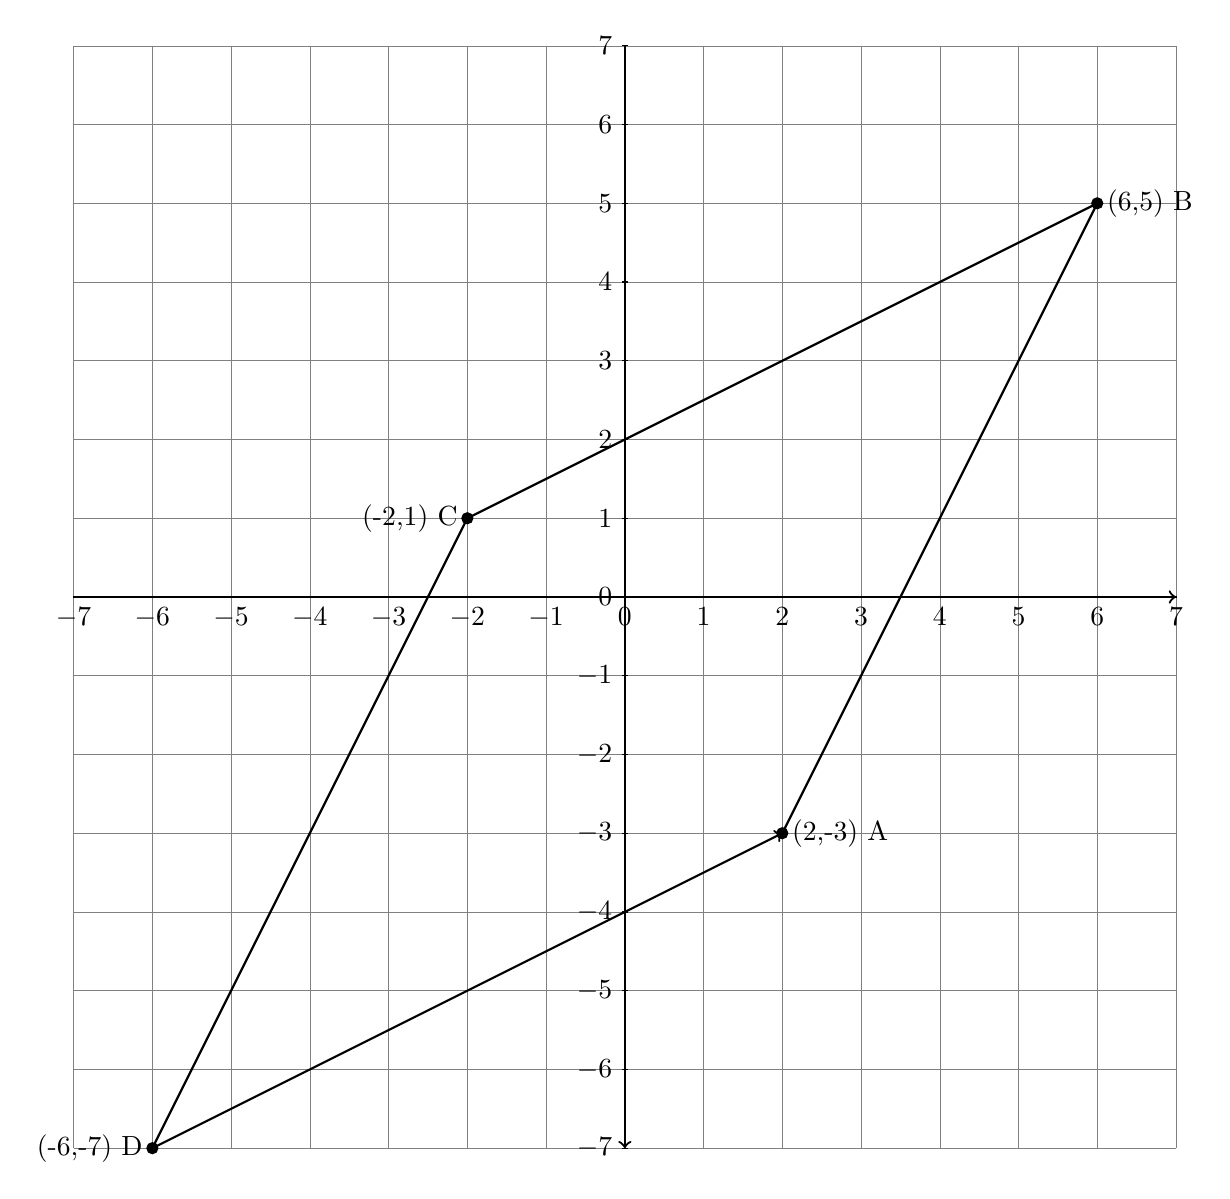
\begin{tikzpicture}
\draw[step=1cm,gray,very thin] (-7,-7) grid (7,7);
\foreach \x in {-7,-6,-5,-4,-3,-2,-1,0,1,2,3,4,5,6,7}
   \draw (\x cm,0.5pt) -- (\x cm,-0.5pt) node[anchor=north] {$\x$};
\foreach \y in {-7,-6,-5,-4,-3,-2,-1,0,1,2,3,4,5,6,7}
    \draw (1pt,\y cm) -- (-1pt,\y cm) node[anchor=east] {$\y$};
\draw[thick,->] (-7,0) -- (7,0);
\draw[thick,->] (0,7) -- (0,-7);
\draw[thick,->] (2,-3) -- (6,5) -- (-2,1) -- (-6,-7) -- (2,-3);
\filldraw[black] (2,-3) circle (2pt) node[anchor=west] {(2,-3) A};
\filldraw[black] (6,5) circle (2pt) node[anchor=west] {(6,5) B};
\filldraw[black] (-2,1) circle (2pt) node[anchor=east] {(-2,1) C};
\filldraw[black] (-6,-7) circle (2pt) node[anchor=east] {(-6,-7) D};
\end{tikzpicture}
\end{document}